\chapter{设计描述}
\label{design-description}

\begin{remark}\color{blue}
The description section defines what the design is. If you find yourself adding rationale, or discussing design alternatives, you are writing text that should be moved into the Development section. A few teams find that this section fits more naturally if it comes before the Design Development section.

In the Fall quarter, the design will be in an early stage and this section is largely a proposal for what the design should be (you can call it that, explicitly). Even so, on the basis of preliminary need-finding, benchmarking and critical function evaluation, you have some idea of what is appropriate. Take a point of view and assert it. A CAD model or systems diagram of a concept may be appropriate.
\normalcolor \end{remark}

\section{设计前景}
\label{设计前景}

\begin{remark}\color{blue}
Use this section to describe your vision or proposal for what you think the design might be. Ideally you should have a sketch, a diagram or other images to help define it.
\normalcolor
\end{remark}

%The remaining text in this section contains of excerpts from the Autodesk 2007-08 Fall document \cite{Autodesk2008Fall}.

为用户提供的功能主要分两方面,远程操作者使用功能,现场机器人提供服务功能。

远程操作界面要集成一系列的应用功能。现场机器人要有足够多的自由度、传感器,确保提供服务的全面性、安全性。

\section{机器人CFP}

%The tactile messaging system was comprised of small Jameco vibrating motors (1.3VDC 8,500 RPM) mounted to ball point pens and wrist patches. A simple switchable voltage supply circuit was created to give each vibrating motor a high (1.2V) and low (0.6V) vibrating speed (\ref{fig:tactile_circuit}). Each voltage level was buffered with LM324 opamps, and the circuits were implemented on protoboards. The high and low speeds were selected by switches. 

移动机器人要能够充分实现操作者所需要的行动功能、音视频获取功能的一系列仿人类的功能。

\begin{itemize}
\item 摄像头视角:机器人的视觉是远程呈现的最核心部分,因此作为机器人的眼睛——摄像头的视角自然是需要十分关注的,单单一个具有较大视角的摄像头是不够的,我们需要摄像头有几乎360度的自由度,并且可以被用户操作旋转,以达到期望的视频捕捉效果。
\item 机器人高度:移动底座与机器人“头部”的连接应该采用可以提供直线位移的推杆类结构,确保与现场的人员交互时能够达到比较好的效果。
\item 
机器人的角度:机器人面向的方向不应该由前进方向单一锁定,在高度可以调整的基础上,我们希望能够让机器人的面部能够在一定的控制下有充分的角度可调,甚至可以是全方位的周角。
\item 
交互界面:机器人的交互界面应该是由远程操作者来控制的,比如对话交流的时候,可以显示操作者的面部图像,使得现场人员感觉更加自然一些;在需要现场帮助的时候,例如操作者想去某个位置,但是由于对现场的陌生,无法立刻确认正确的站点,这时可以求助时,在屏幕上显示区位平面图,如果屏幕是可点击的触摸屏,现场人员直接就可以通过点击帮助远处的操作者选定位置。
\item 
传感器:机器人结构外围应该布置有数量足够的传感器,用以保证机器人安全,并且辅助行动。
\end{itemize}

\begin{figure}[h] 
        \begin{center}
                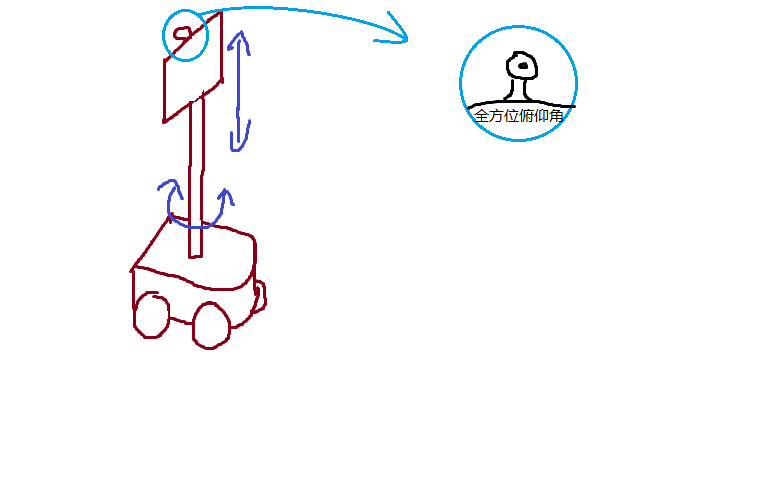
\includegraphics[width= \figwidth]{Figures/ch5.cfp.png}
        \end{center}
        \caption[机器人自由度]{机器人的行动自由度}
        \label{fig:tactile_circuit}  

% \begin{figure}[bhtp] 
%         \begin{center}
%                 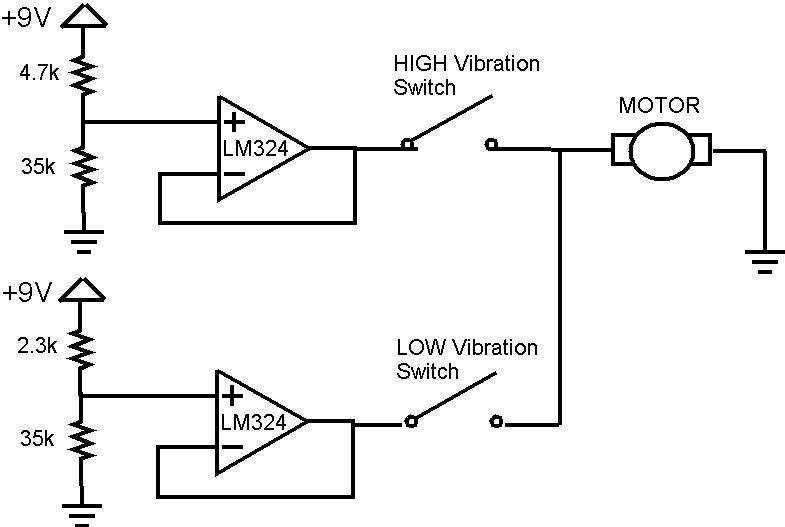
\includegraphics[width= \figwidth]{Figures/Ch5/tactile_circuit.jpg}
%         \end{center}
%         \caption[voltage divider]{A simple voltage dividing circuit provided 1.2V (HIGH) and 0.6V (LOW) buffered output voltages for the vibrating motor. Switches triggered the high and low voltages. }
%         \label{fig:tactile_circuit}  
% \end{figure}

% \begin{center}
% \color{blue}
% (Text omitted for brevity)
% \normalcolor
% \end{center}

% Four independent circuits were created to provide messaging to two motors on each side. 90' 16-gauge wire was passed between two stations in the meeting setup shown in \ref{fig:tactile_seating}. Power supplies provided the 9V signal on each side.

% \begin{figure}[bhtp] 
%         \begin{center}
%                 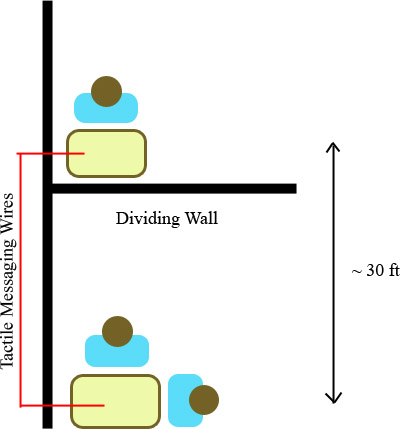
\includegraphics[width=3in]{Figures/Ch5/tactile_seating.jpg}
%         \end{center}
%         \caption[test meeting layout]{Layout of seating during test meeting. Two participants met on one side, with the remote user separated by a wall 50 ft away. }
%         \label{fig:tactile_seating}  
\end{figure}

% In addition to the tactile hardware, Skype was used for video and audio communication. Video was supplied by standard webcams. We mounted the webcams on risers to show video of a sheet of white paper used as the shared drawing space. We chose to focus the video on ideas rather than facial expressions. 


\clearpage
\section{操作网页CFP}

呈献给远程操作者的操作界面是提供远程参观、导航的一个至关重要的接口。该网页界面集合了本系统所有的远程服务功能。

\subsection{数据接口}

%The participation moderator was created by using pre-made desktop software applications called widgets. The desktop was set to a white image, with personal spaces for each participant mapped off by a black boundary and labelled with the participant name. In each personal space, a unique Yahoo! Widgets timer was placed. Unique timer's were used to foster a sense of identity- when glancing at the moderator, the team members could instantly recognize their widget rather than look for their name. 
包括视频传输,音频传输,控制指令采集、传输,反馈信息传输等方面。

视频传输的实时性是主要方面,在网络有延迟的情况下,可以适当牺牲视频品质,
确保流畅、实时的特点。HTML5标准中的WebRTC特性十分符合这个要求。经过简
单测试,发现通过WebRTC,浏览器可以实时地通过浏览器看到摄像头捕获的内容。

音频传输与视频传输要保证一定的同步性。

控制指令的数据量较小,其主要的关注点在于可靠性,保证用户的每个指令都能可靠送达,并且不会由于网络的延迟而误导操作者进行误操作,比如当网络拥堵,用户发送了许多前进的指令,但是机器人接收时有丢包的现象,如果单单是累计确认指令的到达,由于TCP数据包本身的特点,会一并将累积的指令延迟后转入进程,从而使得机器人突然加速前进,造成事故。

另一个方面是控制指令的采集方式,比如敲击键盘,点击按钮,摆动摇杆等操作方式,这些操作依据用户喜好而定,用以增强用户体验。由于直接控制底层的前进、后退等指令对于某些用户过于“危险”,我们可以在界面上提供相应的平面图,并在平片图上设立相应的可点击的“站点”,用户通过点击这些站点,由已经存储的内置路线来操纵机器人相应的移动,并结合传感器来进行相应的避障行走甚至路线修正。

反馈信息是方便用户了解机器人的各项情况,用以辅助操作者进行相应处理。

% \begin{figure}[htbp]
%         \centering
%                 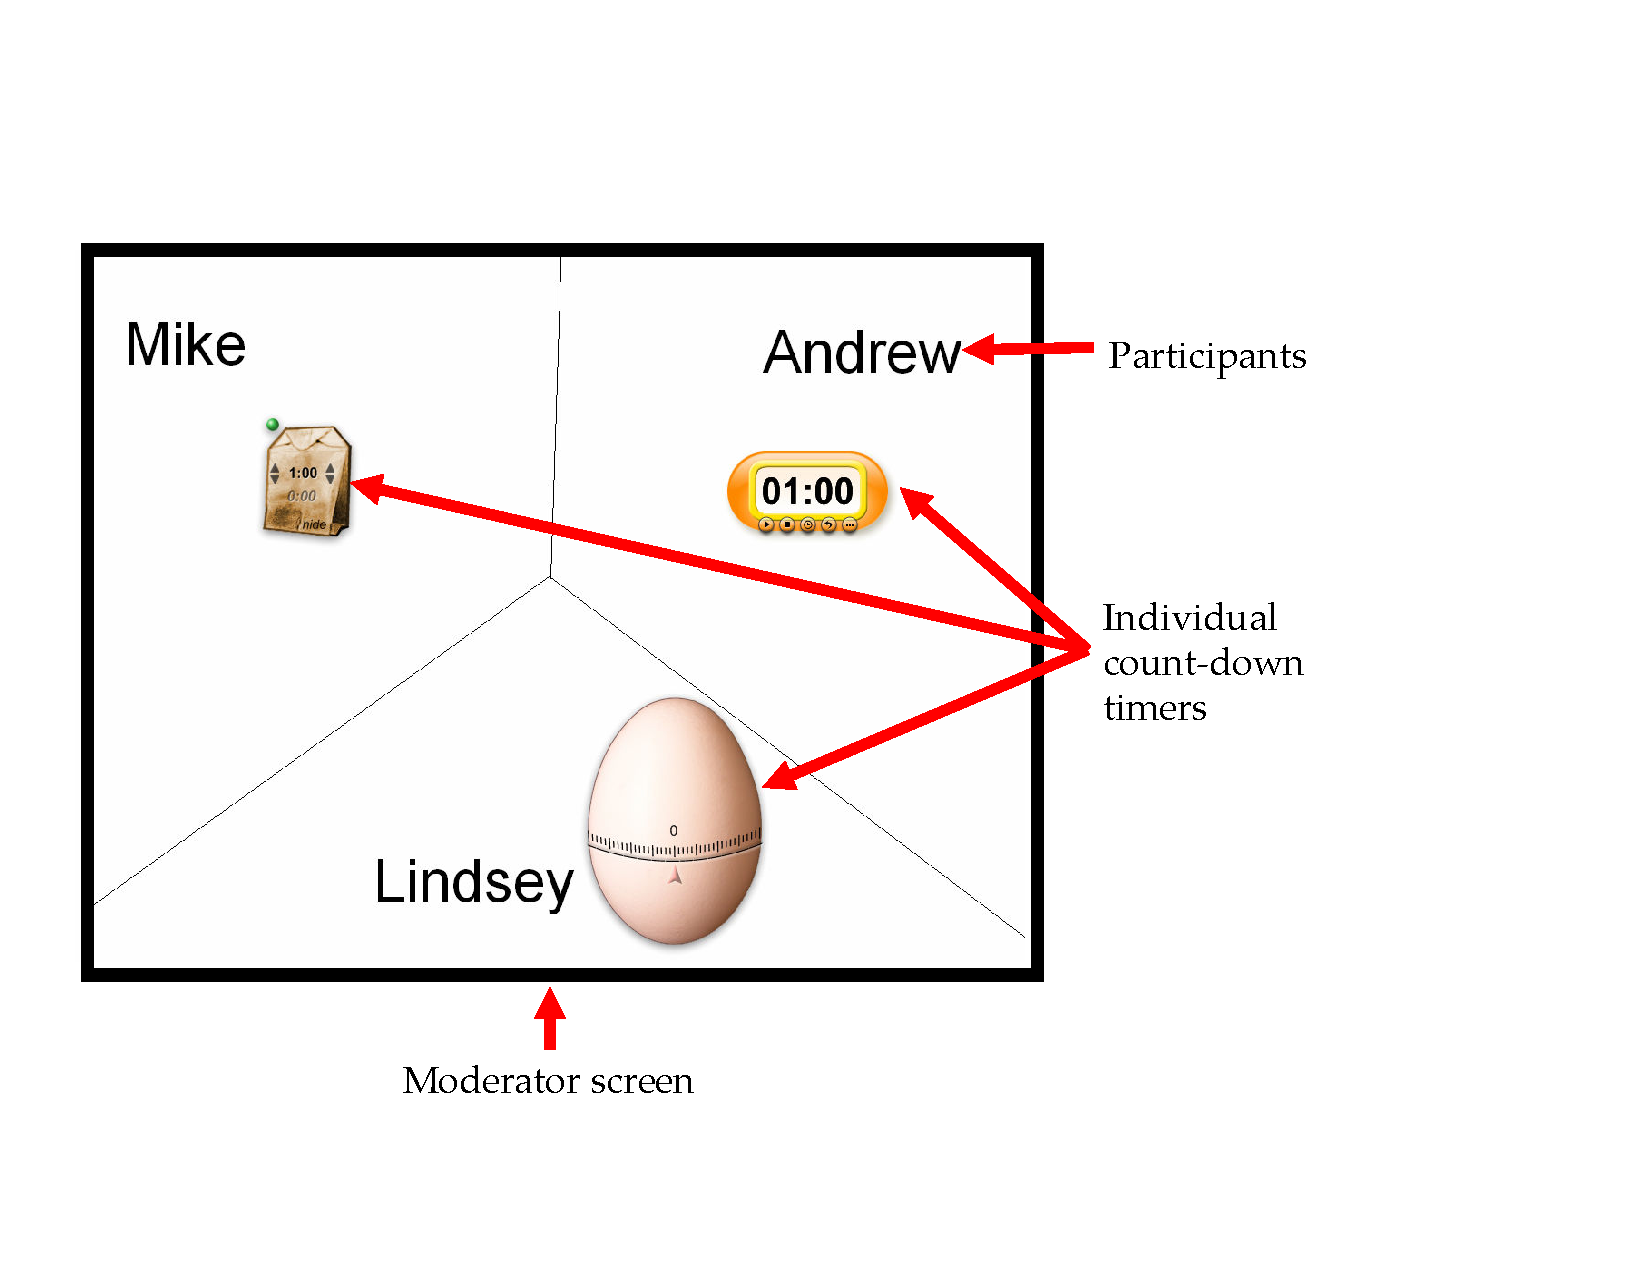
\includegraphics[width=1.00\textwidth]{Figures/Ch5/moderator.pdf}
%         \caption{View of moderator display}
%         \label{fig:moderator}
% \end{figure}

% \begin{center}
% \color{blue}
% (Text omitted for brevity)
% \normalcolor
% \end{center}


% Each was simply a countdown timer with a default starting time, $t_{s}$. As they begin counting down, the amount of time remaining is visible. By clicking twice on any widget, it would reset and begin counting down again from $t_{s}$. The timers were manually reset by one of the teammates during the meeting whenever someone had an interaction. When any timer runs out, it would sound an alarm, designating that the meeting come to a halt until the non-active team member contributes to the conversation. The hypothesis was that, because the timers were visible to the entire team, each member would consciously make an effort to speak before their timer ran out and that no timer would actually buzz, although the rotation of speakers would greatly increase.

% The moderator screen was displayed on a 32" LCD display that was positioned 6' from the center of a table where the group met. The layout is detailed in Figure \ref{fig:moderator_setup}. No video or audio conferencing was used -- all team members were local. The objective of the moderator is to support dialogue in meetings, regardless of whether the members are distributed or not. Audio was recorded of each meeting using Cubase software and an IBM laptop's internal microphone, which was placed in the center of the table so each participant could be heard. 

% \begin{figure}[h]
%         \centering
%                 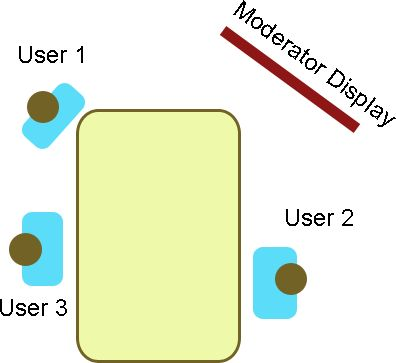
\includegraphics[width=.75\textwidth]{Figures/Ch5/moderator_setup.jpg}
%         \caption{Layout of design meeting with moderator prototype}
%         \label{fig:moderator_setup}
% \end{figure}

\subsection{权限设置}

% Three meetings were run to test the moderator. The subject of each was the same - our team brainstormed potential final products knowing the key lessons learned after our benchmarking. Three meetings were run in succession, each lasting 30 minutes. The intention of this was to eliminate any personal changes between meetings. For example, if Mike has a really bad day before coming in for a second meeting, he may be much less talkative than in the previous meeting, but not as a result of the moderator. The first meeting served as the control, and no moderator was used. The two subsequent meetings used the moderator with $t_{s}$ at 2 minutes and 1 minute.

% The audio files were analyzed manually by playing back the audio recordings for each meeting and recording the length of each comment that every person made. Fifteen minutes of audio during the middle of each meeting was processed. The data are available in Appendix \ref{sec:Appendix1}. 


不同的用户通过登录来进入使用界面,但是用户是广泛的,我们无法直接管理每个用户的操作,故应该采取一定的权限设置,不同的使用者应该具有不同的使用权限。

比如我们完全信赖的人(我们的工作人员)能够直接操作机器人的各个基本功能,合法的用户不能直接控制机器人的底层移动,但是能够通过部分规定好的路线发出指令是机器人沿线行走,此种服务便会使用到之前陈述的可点击平面图的构想,同时,该类用户能够使用摄像头旋转、俯仰等没有涉及到机器人安全的器件的功能。而陌生的游客便只能通过接受视频等简单地信息来使用远程服务,而不能进行其他的使用操作,如此分级使得机器人的使用变得安全化、高效化。
